\section{Random Graph Analysis}\label{sec:random}

This section describes the random graph analysis used in this research.  The testbed, custom graph software, and
the results obtained for the proposed algorithm are discussed.  It finishes with a runtime duration comparison
between the Christofides/Wang, the Zykov, and the proposed algorithm in the target range of \(20\) vertices and
moderate edge density.

\subsection{The Testbed}\label{sec:sub:testbed}

All of the random graph analysis in this research was performed on an Acer Aspire running 64-bit Ubuntu Linux.  The
system contains 8 i7-7780 3.6GHz cores and 20Gb of memory.  The graphing software was custom written in C++.
Although many present day researchers may choose Java or Python, the author feels that the interpretive nature of
those languages combined with unpredictable garbage collection leads to overly inflated and inconsistent results.

The representation of a graph in memory needs to convey the list of vertices, the list of edges, and the connection
matrix.  Graph mutations that change the number of vertices are complex because the connection matrix must be
rebuilt from the altered vertex and edge lists.  Thus, the testbed software assumes that graphs are invariant with
respect to vertex removals and contractions; if vertex removal or contraction is desired then a new graph instance
must be constructed.  Edge additions are innocuous: the new edge can be marked in the connection matrix and
appended to the edge list.

The general layout of a graph instance in memory is shown in \figurename~\ref{fig:layout}.  The vertex and edge
lists are vectors of instances that contain the needed vertex and edge attibutes.  In a particular graph, a vertex
or edge is identified by its position in its list, called its number: vertex numbers are from \(0\) to \(n-1\) and
edge numbers are from \(0\) to \(m-1\).  The connection matrix is a two-dimensional matrix indexed by vertex
numbers: entry \(M[i,j]\) returns a list of edge numbers that can be used to index the edge list to locate the
edges.  If the edge list is empty then the two vertices are not adjacent.  Note that for simple graphs, each edge
list has at most one entry and the connection matrix is symmetric: \(M[i,j]=M[j,i]\).

\begin{figure}[H]
  \centering
  \begin{tikzpicture}[node distance=0in]
    \node (c) [draw, rectangle, minimum height=1in, minimum width=1.5in] at (0,0)
          {\begin{tabular}{c} connection \\ matrix \end{tabular}};
    \node (v) [draw, rectangle, minimum height=1in, minimum width=1.5in, below=of c]
          {\begin{tabular}{c} vertex \\ list \end{tabular}};
    \node (e) [draw, rectangle, minimum height=1in, minimum width=1.5in, below=of v]
          {\begin{tabular}{c} edge \\ list \end{tabular}};
    \node (t) [draw, rectangle, minimum height=1in, minimum width=1.5in, below=of e]
          {\begin{tabular}{c} vertex \\ lookup \\ table \end{tabular}};
  \end{tikzpicture}
  \caption{Graph layout in memory.}
  \label{fig:layout}
\end{figure}

One of the complications of graph mutations is that the vertex and edge numbers change when a new graph is
constructed.  This is why graph mutations result in new instances.  In order to be able to identify vertices across
graph mutations, each vertex is assigned a unique vertex ID when a new graph is created.  Vertices keep their
original IDs across graph mutations, although their numbers may change.  Thus, edges in the edge list refer to
their endpoint vertices by ID and a vertex ID to vertex number lookup table is included as part of the graph
schema.

Contracted vertices are assigned new vertex IDs when created; however, graph algorithms like the proposed algorithm
may need to remember the original vertices that were contracted.  To support this, each vertex instance includes a
list of contracted vertex IDs.  When two non-contracted vertices are contracted, the new contracted vertex has a
contracted vertex ID list consisting of the original two vertex IDs.  When contracted vertices are are contracted,
their contracted vertex ID lists are concatenated.  Thus, contracted vertex ID lists contain only vertex IDs from
the original graph.

One of the most important parameters used by graph algorithms is vertex degree.  As was explained in
\sectionname~\ref{sec:sub:adjacency}, the degree of vertex \(v_i\) can be calculated by summing the \(i^{th}\) row
or column in the connection matrix.  So that degrees do not have to be recalculated each time they are used, the
connection matrix precalculates vertex degrees upon graph creation: each time an edge is added the degrees of the
endpoint vertices are incremented.  The minimum and maximum degrees for a graph still need to be recalculated each
time, so algorithms should cache those values once fetched.

Since new graphs may be created many times during the execution of a graph algorithm, graph construction must be
as efficient as possible.  The testbed software creates a new graph using the following steps:
\begin{enumerate}
\item Each of the \(n\) vertices are added to the new vertex list and a corresponding entry is added to the vertex
  ID to number lookup table.
\item An empty \(n\times n\) connection matrix is allocated with all vertex degrees set to \(0\).
\item Each edge is added to the edge list.  The endpoint vertex IDs are found in the lookup table and the edge is
  registered in the connection matrix, which increments the degrees for the endpoint vertices.
\end{enumerate}

The runtime complexity for new graph construction ignoring memory allocation is determined as follows:
\begin{itemize}
\item Appending a vertex onto the vertex list is \(\BO(1)\).
\item Since the C++ map type is implemented using red/black self-balancing trees, inserting a new vertex into the
  lookup table is \(\BO(\log(n))\).
\item Appending an edge onto the edge list is \(\BO(1)\).
\item Finding each edge's two endpoint vertex numbers in the lookup table is \(\BO(\log(n))\).
\item Adding the edge to the connection matrix and incrementing the endpoint vertex degrees is \(\BO(1)\).
\end{itemize}

The worst case is a complete graph with on the order of \(n^2\) edges.  Therefore, the runtime complexity for
constructing a new graph is \(\BO(n^2\log(n))\).

\subsection{Runtime Complexity Results}\label{sec:sub:runtime}

The proposed algorithm was executed on random graphs for binomial edge probabilities of \(10\%\) to \(90\%\) in
\(10\%\) steps and graph orders of \(5\) to \(30\).  \(1000\) trials were performed per edge probability for graph
orders less than \(20\).  For \(20\) or more, the number of trials was reduced to \(100\) due to increased runtime
duration.  The mean number of calls (\(\log\) base \(2\)) to the recursive method, and hence the mean number of
Zykov tree states traversed, is shown in \figurename~\ref{fig:qzcalls}.

\begin{figure}[H]
  \centering
  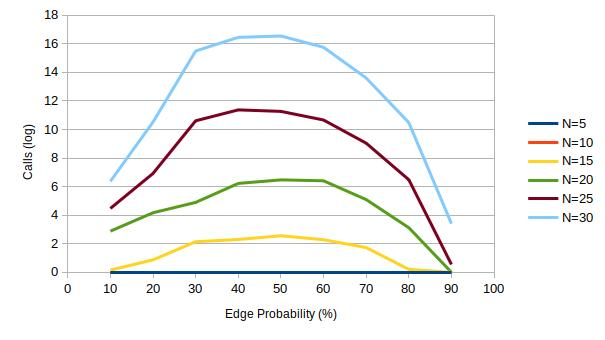
\includegraphics[width=5in]{qz_calls}
  \caption{Proposed algorithm mean number of calls.}
  \label{fig:qzcalls}
\end{figure}

When \figurename~\ref{fig:qzcalls} is compared to the Christofides/Wang results in \figurename~\ref{fig:cfcalls},
it can be seen that for both algorithms the number of calls increases with graph order and peaks with edge density
of \(50\%\).  The bounding tests in the proposed algorithms appear to be effective, resulting in a noticable
decrease in the mean number of states traversed of as much as \(85\%\).

\figurename~\ref{fig:qzruntime} shows the maximum number of calls (log base 2) for each order at \(50\%\) edge
possibility.  A polynomial curve fit to the data indicates a runtime complexity of about
\(\BO(2^{0.0148})\approx\BO(1.0103^{n^2})\).

\begin{figure}[H]
  \centering
  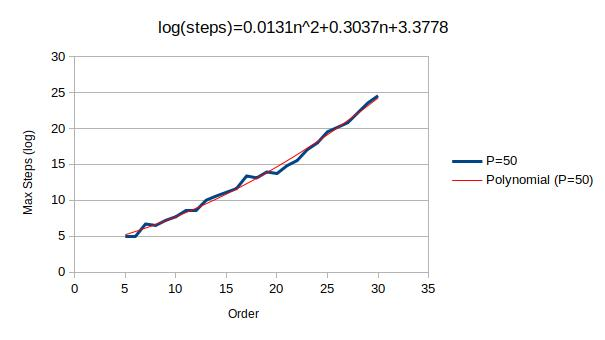
\includegraphics[width=5in]{qz_runtime}
  \caption{Proposed algorithm runtime complexity.}
  \label{fig:qzruntime}
\end{figure}

When \figurename~\ref{fig:qzruntime} is compared to the Christofides/Wang results in
\figurename~\ref{fig:cfruntime}, it can be seen that Christofides/Wang runtime complexity is a bit better:
\(\BO(1.0045^{n^2})\) versus \(BO(1.0103^{n^2})\).  This means that even though the proposed algorithm performs
better in the target range, it will eventually lose to Christofides/Wang.  Based on the equations for the two curve
fits, the break-even point appears to be at about \(n=37\).

\subsection{Bounding Test Results}\label{sec:sub:bounding}

An examination of the effectiveness of the various bounding tests explains why the proposed algorithm eventually
loses to Christofides/Wang.  There are six such bounding tests:
\begin{enumerate}
\item Chromatic number lower/upper bound comparison
\item Maximum edge threshold
\item Small vertex removal
\item Neighorhood subset contraction
\item Minimum common neighbors upper bound
\item Standard Zykov bounding
\end{enumerate}

The frequency with which the Bron Kerbosch estimated chromatic number lower bound and the greedy estimated chromatic
number upper bound match is shown in \figurename~\ref{fig:qzmatch}.  This test is extremely effective at lower orders
but seems to become a non-factor for \(n>25\).

\begin{figure}[H]
  \centering
  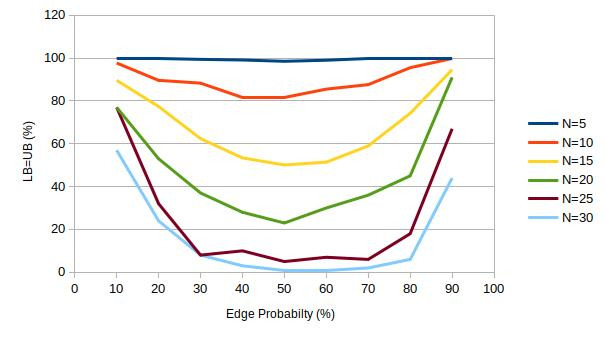
\includegraphics[width=5in]{qz_match}
  \caption{Proposed algorithm lower/upper bound matching test.}
  \label{fig:qzmatch}
\end{figure}

The effectiveness of the maximum edge threshold hits, measured as hits/tries, is shown in
\figurename~\ref{fig:qzedges}.  This test rapidly becomes a non-factor at higher orders; however, since it is a
simple \(\BO(1)\) calculation it is still worth doing.

\begin{figure}[H]
  \centering
  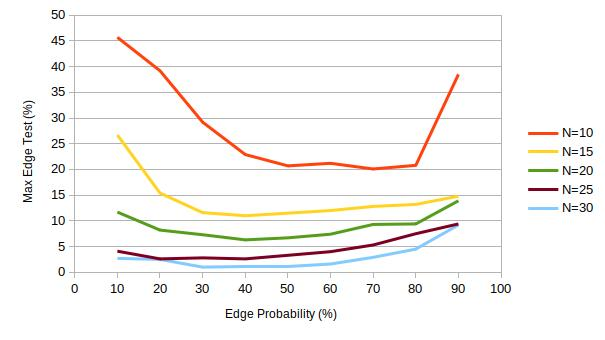
\includegraphics[width=5in]{qz_edges}
  \caption{Proposed algorithm maximum edge threshold test.}
  \label{fig:qzedges}
\end{figure}

The effectiveness of removing small degree vertices, measured as hits/tries, is shown in
\figurename~\ref{fig:qzsmall}.  This test rapidly becomes a non-factor at higher orders.  This is expected because
vertex contraction and edge addition result in degree increases, so no new small degree vertices are ever exposed
once branching begins.  Since the test requires an \(\BO(n)\) scan of the vertices it is still pretty cheap, but is
a candidate for elimination outside of the target range of \(n<20\).

\begin{figure}[H]
  \centering
  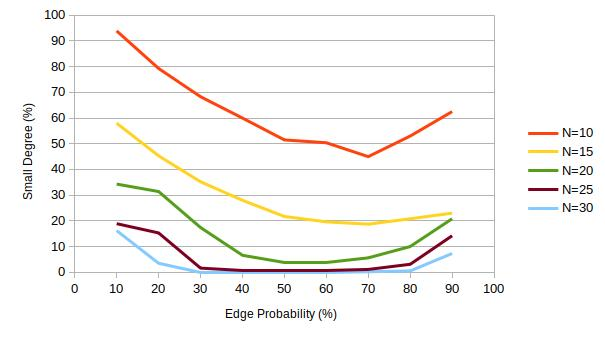
\includegraphics[width=5in]{qz_small}
  \caption{Proposed algorithm small degree vertex test.}
  \label{fig:qzsmall}
\end{figure}

The effectiveness of contracting neighborhood subsets, measured as hits/tries, is shown in
\figurename~\ref{fig:qzsubset}.  This test appears to maintain a decent level of effectiveness at higher orders.
The is not so surprising because more vertices and edges provide more subset opportunities.

\begin{figure}[H]
  \centering
  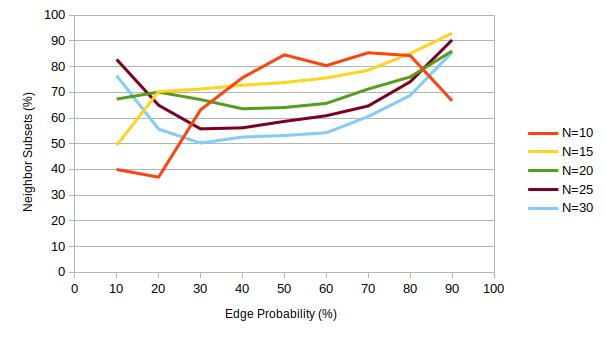
\includegraphics[width=5in]{qz_subset}
  \caption{Proposed algorithm neighborhood subset test.}
  \label{fig:qzsubset}
\end{figure}

The effectiveness of the minimum common neighbors upper bound test, measured as hits/tries, is shown in
\figurename~\ref{fig:qzcommon}.  This test becomes a complete non-factor at higher orders; however, it is based on
the same \(\BO(n^2)\) calculation step required for the more effective neighborhood subset test and only adds an
additional \(\BO(1)\) calculation.  Thus, this test should only be retained if the neighborhood subset test is
retained.

\begin{figure}[H]
  \centering
  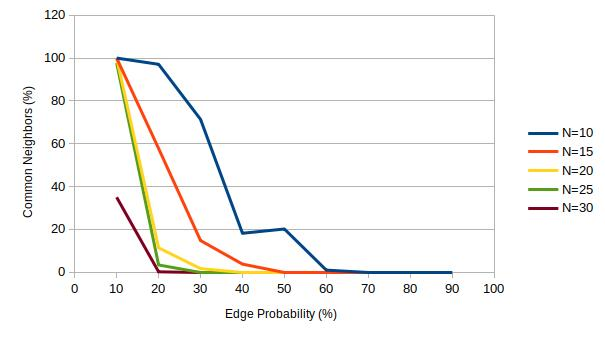
\includegraphics[width=5in]{qz_common}
  \caption{Proposed algorithm minimum common neighbors upper bound test.}
  \label{fig:qzcommon}
\end{figure}

Finally, the effectiveness of the standard Zykov bounding test, measured as hits/tries, is shown in
\figurename~\ref{fig:qzcommon}.  This is the test that uses the Edwards Elphick algorithm to calculate a new
chromatic number lower bound and prune if that value exceeds the current value of \(k\).  This test appears to have
increased effectiveness at higher orders.

\begin{figure}[H]
  \centering
  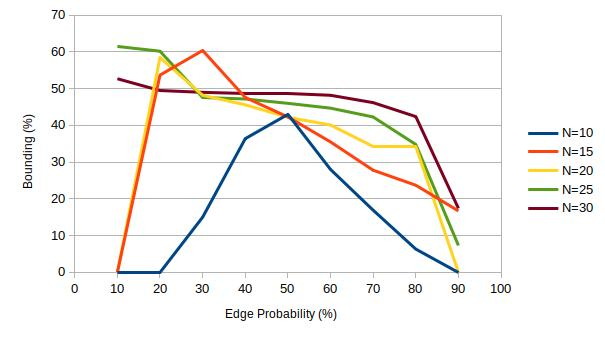
\includegraphics[width=5in]{qz_bounding}
  \caption{Proposed algorithm bounding test.}
  \label{fig:qzbound}
\end{figure}

\subsection{Runtime Duration Results}

\begin{figure}[H]
  \centering
  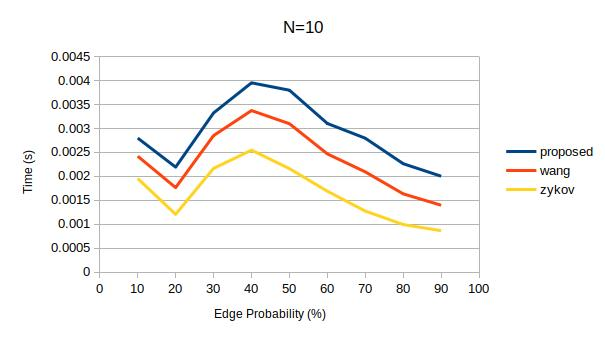
\includegraphics[width=5in]{duration_10}
  \caption{Runtime durations at \(n=10\).}
  \label{fig:duration10}
\end{figure}

\begin{figure}[H]
  \centering
  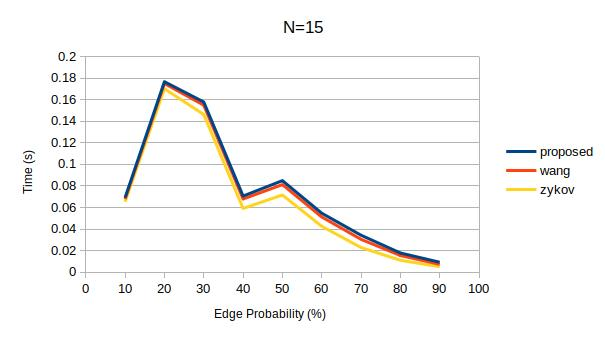
\includegraphics[width=5in]{duration_15}
  \caption{Runtime durations at \(n=15\).}
  \label{fig:duration15}
\end{figure}

\begin{figure}[H]
  \centering
  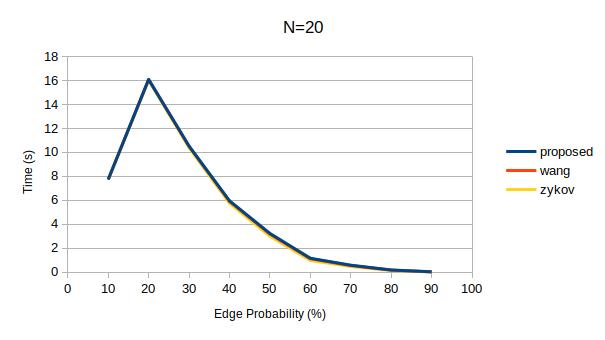
\includegraphics[width=5in]{duration_20}
  \caption{Runtime durations at \(n=20\).}
  \label{fig:duration20}
\end{figure}
